% This is samplepaper.tex, a sample chapter demonstrating the
% LLNCS macro package for Springer Computer Science proceedings;
% Version 2.20 of 2017/10/04
%
\documentclass[runningheads]{llncs}
%
\usepackage{graphicx}
\usepackage[portuges]{babel}
\usepackage[T1]{fontenc}
\usepackage{verbatim}
\usepackage{float}
\usepackage{caption}
\usepackage[hidelinks]{hyperref}
%Path relative to the .tex file containing the \includegraphics command
\graphicspath{ {./images/} }
% Used for displaying a sample figure. If possible, figure files should
% be included in EPS format.
%
% If you use the hyperref package, please uncomment the following line
% to display URLs in blue roman font according to Springer's eBook style:
% \renewcommand\UrlFont{\color{blue}\rmfamily}
\setcounter{secnumdepth}{6}
\renewcommand\theparagraph{\Alph{paragraph}}
 
\makeatletter
\renewcommand\paragraph{\@startsection{paragraph}{4}{\z@}%
                                      {-3.25ex\@plus -1ex \@minus -.2ex}%
                                      {0.0001pt \@plus .2ex}%
                                      {\normalfont\normalsize\bfseries}}
\renewcommand\subparagraph{\@startsection{subparagraph}{5}{\z@}%
                                      {-3.25ex\@plus -1ex \@minus -.2ex}%
                                      {0.0001pt \@plus .2ex}%
                                      {\normalfont\normalsize\bfseries}}
 
\counterwithin{paragraph}{subsubsection}
\counterwithin{subparagraph}{paragraph}
\makeatother
\hyphenation{ProcessID}
\begin{document}
%
\title{PDF PAdES (DSS \& CMD) Signature Command Line Program}
%
\titlerunning{PDF PAdES - Signature Command Line Program}
% If the paper title is too long for the running head, you can set
% an abbreviated paper title here
%
\author{ Henrique José Carvalho Faria nº82200 }
%
% First names are abbreviated in the running head.
% If there are more than two authors, 'et al.' is used.
%
\institute{Departamento de Informática, Universidade do Minho}
%
\maketitle              % typeset the header of the contribution
%
% Abstract
\begin{abstract}


Neste trabalho foi pedido que se emulasse o programa \textit{PDF PAdES} desenvolvido pela empresa \textit{DeviseFutures} em \textit{Perl}. Adicionalmente, este programa deve aplicar medidas de segurança que previnam diversos ataques que visem compromenter o funcionamento do sistema ou tirar partido do mesmo para obter informações. Assim, a ordem de trabalhos passou por realizar um estudo das vulnerabilidades a que o programa está sujeito seguindo-se o desenvolvimento do programa validando cada input recebido tendo em conta as vulnerabilidades a que este está sujeito.
Este relatório começa por descrever o processo de emulação da aplicação e posteriormente realiza uma sumula das vulnerabilidades possíveis e de que forma foram tratadas.


\keywords{Perl \and Buffer-Overflow \and String Vulnerabilitys \and Integer Vulnarabilitys \and Input Validation \and white List \and Black List}
\end{abstract}
%
%

\newpage
\newpage
\hfill
% Aqui começam os capitulos abordados pelo trabalho
\section{Criação da aplicação PDF PAdES em Perl}

Para este trabalho seguiu-se a estrutura do programa original separando o corpo da aplicação, que ficou no ficheiro signpdf\_cli.pl, das operações sobre ficheiros, chave móvel e ligação ao servidor SOAP, que ficaram no modulo cmd\_soap\_msg.pm, das operações realizadas por um servidor REST que se colocaram num módulo chamado dss\_rest\_msg.pm, e das variáveis APPLICATION\_ID e DSS\_REST que ficaram no modulo cmd\_config.pm. Adicionalmente foi criado um módulo para tratamento de segurança da aplicação chamado \textit{verifiers.pm}.\newline


Para o corpo do programa o Perl começa por importar as variáveis \textit{\$APPLICATION\_ID} e \textit{DSS\_REST} do modulo \textit{signpdf\_config} através das subrotinas \textit{get\_appid()} e \textit{get\_rest()} respetivamente. Caso a variável \textit{\$APPLICATION\_ID} não esteja definida o programa termina. \newline

Em seguida é verificado se o programa foi invocado com argumentos, caso contrário o programa também termina informando o utilizador que deve utilizar o comando \textit{signpdf\_cli.py [-h]} para obter ajuda sobre como funciona o programa. Caso tenha sido invocado com argumentos é realizado um parser dos dados recorrendo ao módulo \textit{Getopt::Long} que faz uso de flags para identificar inequivocamente cada variável recebida como parâmetro. Em seguida estes argumentos são colecionados num array cujas variáveis definidas serão verificadas fazendo uso das subrotinas pertencentes ao módulo \textit{verifiers.pm}.\newline
Caso o input passe nas verificações de segurança, é dado inicio ao processo de assinatura do pdf recorrendo á chave móvel digital.\newline
Convêm referir que, ao contrário do que foi realizado no ficheiro original \textit{signpdf\_cli.py} as verificações de segurança referentes ao código das mensagens recebidas do servidor foram realizados no módulo \textit{cmd\_soap\_msg.pm}.

\subsection{Módulos}

Para instalar os módulos necessários pode-se utilizar uma ferramenta chamada \textit{cpanm}. Pode-se descarregar esta ferramenta para linux com o comando de terminal \textit{sudo apt install cpanminus}.\newline
Após instalar a ferramenta deve-se garantir que se têm os seguintes módulos instalados\footnote{Nota: Para descarregar os módulos use no terminal o comando cpanm install 'nome do módulo'}:

\begin{enumerate}
	\item Crypt::OpenSSL::X509
	\item DateTime
	\item Digest::SHA
	\item MIME::Base64
	\item Getopt::Long
	\item POSIX
	\item List::MoreUtils
	\item Carp
	\item FindBin
	\item IO::Prompt
	\item REST::Client
	\item XML::Compile::WSDL11
	\item XML::Compile::SOAP11
	\item XML::Compile::Transport::SOAPHTTP
	\item Encode
	\item Bit::Vector
	\item HTTP::Request
	\item HTTP::Parser
	\item Log::Log4perl
	\item LWP::ConsoleLogger
	\item strict
\end{enumerate}
\newpage
\section{Vulnerabilidades Gerais}

No desenvolvimento de um software devemos sempre garantir que não divulgamos informação sobre como a nossa aplicação está construida. Durante o deenvolvimento do código deparamo-nos com dois possíveis problemas a tratar.\newline
\par O primeiro problema enuncia-se em seguida, "Como encerrar a aplicação com uma exceção passando uma mensagem de erro ao utilizador sem lhe revelar informação sobre o código da aplicação?". Para resolver este problema usamos a função \textit{die}, o problema é que esta para além da mensagem fornece informação sobre a linha onde ocorreu a exceção. Felizmente caso se adicione \textit{\\n} ao final da mensagem de erro emitida pelo die este omite a informação referente á linha. 
\par O segundo problema encontrado é referente á função \textit{open}, até ao ano 2000, a função open usava 2 parâmetros, um para a variável para a qual se lê e uma para o ficheiro a ler. O problema  acontece caso o utilizador use um ficheiro cujo nome comece, por exemplo, com o sinal \textit{>}, isto levará a que por exemplo caso seja dado como input o ficheiro \textit{>/etc/passwd} nós acabamos de apagar o ficheiro de passwords do Linux. Para resolver este problema usamos a versão do open com 3 variáveis, uma para guardar a informação a ler do ficheiro, uma para o tipo de leitura a realizar no ficheiro e uma para o nome do ficheiro. Acresce a este problema o facto de que caso o open use um pipe em vez de um ficheiro, ao falhar este devolve o pid do subprocesso na mensagem de erro, como queremos evitar divulgar qualquer informação sobre a aplicação usamos então a função \textit{die} para emitir o erro sem comprometer a nossa implementação tomando o código a seguinte forma: \textit{open(variável para leitura, modo de leitura, ficheiro a ler) or die ... }.\newline

\textit{Nota: As restantes questões de segurança foram abordadas e tratadas num modulo perl a parte chamado \textbf{verifiers.pm} criado para separar de forma legivel as subrotinas usadas para segurança das subrotinas do programa principal.}\newline 

Existem enúmeras vulnerabilidades a tratar para além das duas supramencionadas, nomeadamente:
\begin{enumerate}
\item Restrições sobre a memória
\item Neutralização do input durante a geração da página web
\item Improper Input Validation
\item Information Exposure
\item Out-of-Bounds Read
\item Neutralização de elementos especiais para comandos SQL (SQL Injection)
\item use after free
\item Integer Overflow or Wrapparound
\item XML Injection
\item OS Commands Injection
\item SQL Injection
\end{enumerate}

Destas vulnerabilidades a 1ª 4ª, 5ª, 6ª, 7ª e 8ª podem ser ignoradas visto que o \textit{Perl} trata da alocar as variáveis na memória libertando o programador da manutenção da mesma, para além. Assim vamos debruçar-nos sobre a vulnerabilidade 3, 9,10 e 11.


\subsection{Improper Input Validation}

Nesta secção falaremos um pouco dos inputs e da validação realizada sobre os mesmos. A validação de inputs de uma aplicação é fulcral para o bom funcionamento da mesma, nunca devemos acreditar que o utilizador usará a aplicação da melhor forma ou para fins nefastos.\newline


Assim os inputs a verificar são:  o número de telefone, o pin e o nome do ficheiro a assinar. Caso sejam fornecidos, o nome do ficheiro assinado e a data fornecida também serão verificados.\newline

\begin{itemize}
\item Nomes dos ficheiro\newline
 Para realizar a verificação tanto do nome do ficheiro de input como do ficheiro de output o processo aplicado foi o mesmo. Foram criadas 2 listas, uma white list com os caracters aceitaveis para constituirem o nome de um ficheiro (As White Lists são especialmente proveitosas visto que é mais facil indicar o que é aceitavel do que o que não é, em contrapartida limitamos um pouco os nomes possíveis para os ficheiros fornecidos) e uma black list onde removemos algumas hipóteses aceitáveis na white list mas que não podem ser dados como input do nome do ficheiro que são as flags usadas nos inputs do programa.\newline
 Convem notar que tentativas de inserção de vários comandos através da adição de \textit{;} ou de pipes com o caracter \textit{|} não funcionam pois não pertencem á lista de caracters permitidos pela white list.

\hfill\newline
\item Número de telefone\newline
 No caso do número de telefone desenvolvemos 2 regex sendo que um funciona para números internacionais e nacionais e um que funciona apenas para números nacionais, os respetivos regex apresentam-se em seguida:\newline
\begin{itemize}
	\item \textit{/\^{}\textbackslash+[0-9]\{1,3\} [0-9]\{4,14\}\$/}
	\item \textit{/\^{}\textbackslash+351 [0-9]\{9\}\$/}
\end{itemize}

\hfill\newline
\par Como a chave móvel digital para a qual a aplicação se destina normalmente está associada a números de telemovel portugueses mantivemos o segundo regex embora tenhamos deixado em comentário o segundo regex caso pretendamos estender a aplicação a números estrangeiros. A razão de escolhermos apenas números nacionais prende-se com a escolha de implementar uma segurança com granularidade mais fina visto que o número de dígitos de telemovel varia de país para país e o indicativo também.\newline
\textit{Nota: Convém notar que, nas expressões regex, são usados por vezes 2 simbolos, o \^{} no inicio do regex e o \$ no fim. Estes simbolos indicam ao perl que o regex tem de corresponder ao inicio do input e ao final deste respetivamente, isto é, caso ambos os simbolos sejam usados o perl entende que o input a testar tem de ser totalmente formado pelo regex e, caso não seja, falha a verificação.}\newline
\hfill\newline
\item PIN\newline

\par O PIN é um conjunto de 4 a 8 digitos, assim, para o testar bastou um regex simples que garantisse isso: \textit{/\^{}[0-9]\{4,8\}\$/}.

\hfill\newline
\item OTP\newline
\par O OTP é verificado como sendo um conjunto de 6 digitos. Mais uma vez o regex usado é bastante simples: \textit{/\^[0-9]\{6\}\$/}.


\hfill\newline
\item Process ID\newline

\par O ProcessID trata-se de um conjunto de 32 caracters (números e letras) que seguem um padrão especifico de formação com a seguinte caraterística: \textit{XXXXXXXX-XXXX-XXXX-XXXX-XXXXXXXXXXXX}.\newline
\par Desta forma foi criado um padrão regex que permitisse verificar se o ProcessID recebido tinha 32 caracters sendo que este era constituido por conjuntos de 8, 4, 4, 4 e por fim 12 caracters separados por travessões: \textit{/\^[a-z0-9]\{8\}-[a-z0-9]\{4\}-[a-z0-9]\{4\}-[a-z0-9]\{4\}-[a-z0-9]\{12\}\$/}.

\hfill\newline
\item Datetime\newline

\par A Datetime trata-se de uma indicação temporal que respeita uma notação temporal reconhecida pelo servidor \textit{Rest} com o qual a aplicação comunica: \textit{YYYY-MM-DDTHH:MM:SS.SSSSSS}.
\par Para verificar se a data foi inserida respeitando a notação exigida foi criado um regex para a mesma: \textit{/\^\textbackslash d\{4\}-\textbackslash d\{2\}-\textbackslash d\{2\}T\textbackslash d\{2\}:\textbackslash d\{2\}:\textbackslash d\{2\}.\textbackslash d\{6\}\$/}. Este regex verifica se a informação é inserida, com os respetivos simbolos extra\footnote{Simbolos extra: - (separa a informação da data anual), T (separa a informação da data da informação horária), : (separa a informação horária).}, na forma ano, mês, dia, hora, minutos, segundos, nanosegundos.

\hfill\newline
\item Response\newline

\par Ao debruçarmo-nos sobre como validar a Response do servidor convêm notarmos algumas caraterísticas desta que nos podem ajudar a verificar que esta não foi alterada. 
\begin{enumerate}
	\item A resposta tem um tamanho fixo de 560 bytes independentemente do conteudo enviado para o servidor.
	\item A resposta está em base 64, ou seja só possui os seguintes caracters: [a-zA-Z+\/].
\end{enumerate}

\par Á luz desta informação podemos delinear algumas verificações para mitigar o risco de ataques be sucedidos á nossa aplicação.
\par A primeira verificação pasa por confirmar que a Response tem o número de caracters correto, assim não é possível a adição de código extra ao conteúdo da mensagem. A segunda verificação passa por verificar a existência apenas de caracters de base 64 na mesma. Por fim podiamos tentar verificar a existência de sintax SQL ou XML mas tal não será necessário uma vez que não é possível estas existirem visto que, em base 64, não se possuem os caracters: espaço, ponto e virgula, maior, menor entre outros necessários para as mesmas terem uma sintax correta.


\hfill\newline
\item Signature\newline

Mais uma vez á semelhança do parâmetro anterior a Signature tem um comprimento fixo e está em base 64. Assim, as verificações de segurança aplicadas apenas diferem na verificação do tamanho que passa de 560 para 512.


\end{itemize}


O principal foco da segurança na nossa aplicação foi aplicado ás strings. Os critérios usados na \textit{white List} e na \textit{Black List} não são muito restritivos, principalmente porque as strings são maleáveis e o utilizador pode dar o nome que quiser ao documento que pretende utilizar com a aplicação. Desta forma é necessário ter atenção a utilizadores mal intencionados que pretendam usar os critérios laços de filtragem de input para fins diferentes daquele para o qual a aplicação foi feita.\newline


\subsection{OS Injection}

O Perl é relativamente suscetivel a injeção de comandos do sistema operativo, isto pois permite utilizar pipelines com o caracter \textit{|} como input ou comandos seguidos separados pelo caracter \textit{;}. Para ambos os casos existe uma solução que apesar de restringir a liberdade do cliente de nomear os seus ficheiros recorrendo aos caracters \textit{|} e \textit{|} garante que estes ataques não ocorrem, o que do ponto de vista de uma maior qualidade na segurança da aplicação é o ideal.


\subsection{XML Injection}

Nesta subsecção vamos tratar de qualquer tentativa de injeção de código \textit{XML} na nossa aplicação. Para lidar com tentativas de injeção de código \textit{XML} através de um input foi criada uma subrotina chamada {xmlInjection} no modulo \textit{verifiers.pm}.\newline
Nesta subrotina para evitar eventuais tentativas de injeção de código \textit{XML} foi realizado um regex com a forma: \textit{/$<$[a-zA-Z]*($>$[\^{} ($<$\textbackslash/)]*$<$/[a-zA-Z]*|\textbackslash/)?$>$/} . Este regex permite realizar match entre elementos desta linguagem através de sintaxe conhecida detetando padrões como \textit{<qualquer coisa> ... </qualquer coisa>} ou \textit{<qualquer coisa/>}.

\subsection{SQL Injection}

Para tratar eventuais tentativas de injeção de código \textit{SQL} através das variáveis, foi definida uma subrotina chamada \textit{sqlInjection} que possui um array de palavras chave usadas na syntax \textit{SQL} que são comparadas através de um regex com os argumentos. Caso seja detetado num argumento uma palavra pertencente á syntax \textit{SQL} o programa emite uma mensagem de erro a avisar que detetou uma tentativa de SQL injection.

\section{Certificados Falsos}

Um problema quando se lida com certificados prende-se com a validação dos mesmos. De forma a contornar este problema recorreu-se ao módulo \textit{LWP::UserAgent}, este fornece uma opção por defeito de verificação automática do servidor e da sua legitimidade chamada \textit{verify\_hostname}. Assim são escolhidos protocolos seguros e é assegurado que nos ligamos a um servidor que possui um certificado válido.
\newpage
\section{Testes}
\label{sec:Testes}

\par Esta secção divide-se em duas subsecções, a primeira diz respeito a refactoring e identificação de Code Smells\footnote{Code Smell: característica do código fonte ou do programa que pode indicar um problema mais grave.}\cite{codeSmells1,codeSmells2} e a segunda prende-se com testes feitos á aplicação para testar a sua robustez.

\subsection{Refactoring e Code Smells}


\subsubsection{Devel::Cover}
\hfill\newline

\par Para realizar o processo de code coverage foi usado o módulo \textit{Devel::Cover}\cite{develCover}. Este módulo permite correr um programa com os respetivos argumentos e monitorizar que partes do código foram usadas ou não foram usadas, criando posteriormente um relatório em html que permite visualizar de uma forma mais clara o desempenho do programa.
\par Para utilizar o \textit{Devel::Cover} com o nosso programa e posteriormente criar o relatório pretendido basta correr os seguintes comandos pela ordem apresentada:
\begin{itemize}
	\item perl -MDevel::Cover signpdf\_cli.pl -u '+351 XXXXXXXXX' -p XXXX -infile teste.pdf -d
	\item cover
\end{itemize}

Após o programa terminar de executar podemos verificar que foi criada uma base de dados \textit{cover\_db} e que a informação da mesma foi compilada num relatório html.
O resultado de correr o teste\footnote{Note-se que a utilização do -d não é obrigatória mas foi usado para cobrir a maioria do código.} é apresentado em seguida:

\begin{figure}[H]

  \centering
  \captionsetup{justification=centering}

  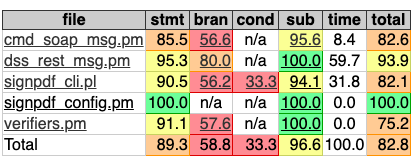
\includegraphics[scale = 0.25]{coverage1.png}
  
  \caption {Resultado de correr o programa utilizando o módulo Devel::Cover}

  \label{fig:coverage1}
\end{figure}


\par Analisando a imagem anterior, verificamos que existem várias colunas na tabela, cada coluna tem o seguinte significado da esquerda para a direita respetivamente: número de linhas do código utilizadas, nº de branches(if/else) utilizados\footnote{O número ótimo de branches utilizados é de 50\% uma vez que quando o código chega a um if then else segue apenas 1 dos caminhos possíveis, no entanto existem partes do código que possuem apenas um if ou que possuem sub-rotinas que não foram chamadas que possuem ifs, estes ifs contam para esta percentagem, fazendo o valor final subir ou descer respetivamente.}, percentagem das condições (as condições são compostas por elementos conjugados com as palavras \textit{and} e \textit{or}) avaliadas de forma positiva ou negativa, percentagem de sub-rotinas usadas, tempo em segundos que as sub-rotinas de cada ficheiro demoraram a executar.
\par Ao analisarmos os ficheiros para verificarmos que "statements" não estão a ser utilizados no código podemos verificar que estes se encontram todos dentro de condições if then else, sendo que como o programa correu bem, os statements não utilizados se encontram dentro dos else. Analisando a utilidade dos "statements" dentro de cada else constatamos que na sua maioria se tratam de comandos \textit{die} com informação sobre o porquê do programa ter sido interrompido naquele estágio, jutificando a sua permanência.


\par Passando agora á análise dos branches do programa, devemos analisar para cada ficheiro se os branches são necessários, ou seja se as condições para que se siga por cada um dos caminhos das biforcações se manifestam. Tomemos por exemplo o relatório referente ao ficheiro \textit{cmd\_soap\_msg.pm}.

\begin{figure}[H]

  \centering
  \captionsetup{justification=centering}

  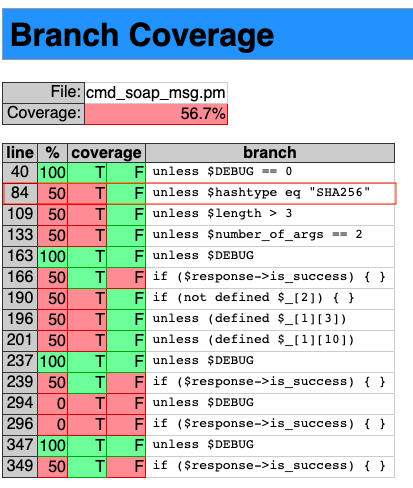
\includegraphics[scale = 0.25]{SOAPcoverage2.png}
  
  \caption {Relatório de branches do ficheiro cmd\_soap\_msg.pm}

\end{figure}

\par Após verificarmos a validade de cada branch, podemos observar que há um branch que não faz sentido porque verifica se um dado valor foi recebido como input dessa subrotina sendo que esse valor é passado de forma estática (esse branch foi assinalado a vermelho para facilitar o seu reconhecimento). Podemos então apagar esse branch uma vez que não tem utilidade no código. O mesmo processo foi aplicado a cada ficheiro, no entanto optou-se por não se mostrar visto que o tratamento é homólogo e não houve mais nenhum caso de uma condição desnecessária.

\par Podemos ainda ver, na figura\ref{fig:coverage1}, que existe uma condição no código. O módulo Devel:Cover cria também um relatório para as condições do programa como se pode ver na imagem abaixo.

\begin{figure}[H]

  \centering
  \captionsetup{justification=centering}

  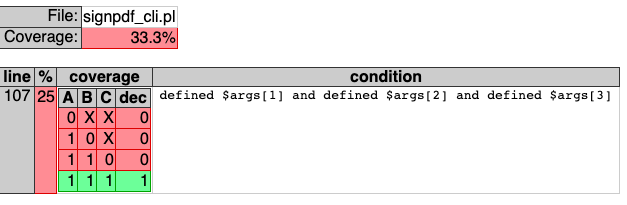
\includegraphics[scale = 0.25]{condition.png}
  
  \caption {Relatório de condições do ficheiro signpdf\_cli.pl}

\end{figure}

Podemos verificar que são mostradas as vária verificações que podem ser levadas a cabo e os respetivos resultados. Estes resultados são todos possíveis porque até aquele ponto não existe verificação se os 3 elementos que o cliente tem de fornecer ao programa são realmente fornecidos.
\par Concluida a verificação de existência de código inútil, confuso, muito extenso ou duplicado confirma-se que o único problema encontrado foi a existência do if que fazia a verificação de um elemento estático do código.


\subsubsection{Perl::Critic}
\hfill\newline

\par Após serem removidos os code Smells do código usou-se uma biblioteca chamada \textit{Perl::Critic}\cite{perlCritic} que avalia o código fonte de acordo com as diretrizes do livro Perl Best Practices\cite{bestpractices}, além de avaliar outras métricas, como a complexidade ciclomática. Este módulo permite escolher 5 tipos de severidade de problemas no código, podendo as falhas mais severas representar problemas que permitam que um utilizador mal intencionado se aproveite do nosso programa e as falhas mais ligeiras apenas questões de legibilidade do código. Por esta razão começamos por definir uma severidade de grau 4, desta forma apenas foram apresentados os erros mais graves, de severidade 5, a vermelho e os segundos mais graves, de severidade 4, a laranja\footnote{Por questões de simplicidade de apresentação apenas é apresentado o resultado da aplicação do módulo ao ficheiro signpdf\_cli.pl, no entanto ressalva-se que o mesmo processo foi aplicado aos restantes ficheiros do programa.}.

\begin{figure}[H]

  \centering
  \captionsetup{justification=centering}

  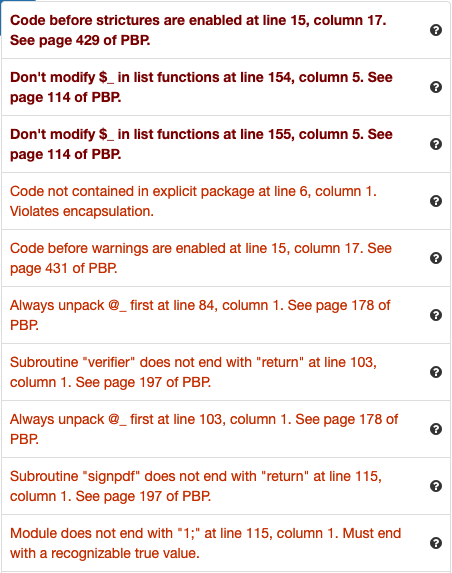
\includegraphics[scale = 0.3]{critic1.png}
  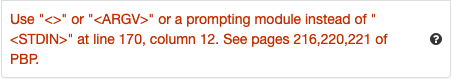
\includegraphics[scale = 0.3]{critic2.png}
  
  \caption {Relatório \textit{Perl::Critic} de gravidades 4 e 5 do ficheiro signpdf\_cli.pl}

\end{figure}

\par As 3 primeiras notificações apresentadas correspondem a problemas críticos no código perl que foram resolvidos adicionando, após a adição do último módulo necessario, \textit{use strict;} para a primeira notificação e para as restantes duas bastou remmover o map que estava a ser usado para modificar uma lista de certificados aplicando um regex substituindo-o pela sub-rotina \textit{apply()} do módulo \textit{List::MoreUtils}\cite{perllist}. As restantes notificações possuem severidade 4. 
\par A primeira notificação refere-se á não identificação do código atual como um package, notificação essa que foi prontamente resolvida indicando na primeira linha do código \textit{package signpdf\_cli;}. A segunda notificação desapareceu com a adição do "use strict;" utilizado para remover a primeira notifiação de severidade 5.
\par Duas das notificações referiam que se trata de uma boa prática copiar o array recebido por uma sub-rotina para uma variável extra e utilizar esta, uma vez que caso o array original seja alterado dentro da sub-rotina, essa alteração \mbox{refletir-se-á} na sub-rotina que a invocou. Adicionalmente 3 outras notificações foram resolvidas adicionando \textit{return 1;} ao final de todas as sub-rotinas que ainda não o possuiam e \textit{1;} no final do ficheiro, visto que os ficheiros em perl devem acabar com um valor de verdade.
\par Por fim o uso de \textit{<STDIN>} foi substituido pelo uso da sub-rotina \textit{prompt} pertencente ao módulo \textit{IO::Prompt}\cite{ioPrompt}.

Como todas as notificações para uma análise de gravidade 4 pareciam importantes, decidi diminuir o filtro de gravidade da análise do ficheiro para 3 e o resultado obtido pode-se ver na imagem abaixo.

\begin{figure}[H]

  \centering
  \captionsetup{justification=centering}

  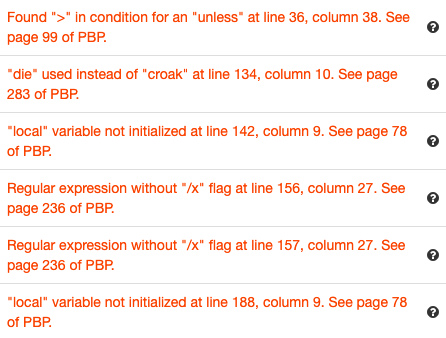
\includegraphics[scale = 0.4]{critic3.png}
  
  \caption {Segundo relatório \textit{Perl::Critic} de gravidade 3 do ficheiro signpdf\_cli.pl}

\end{figure}
\par Estes erros são meramente para melhorar a simplicidade aciclomática do código, ou a legibilidade do mesmo, por esse motivo apliquei as mudanças requeridas ao ficheiro.
\par A primeira notificação referia que ao usar o simbolo de > dentro de um unless implicava uma dupla negativa (trata-se de uma questão de sacrificar velocidade de execução do código por legibilidade), assim foi modificado o código, trocando o unless por um if tornando o código mais eficiente.
\par A segunda notificação apenas pretende assinalar que quando nos deparamos com um erro de input por parte do utilizador, não devemos usar o comando \textit{die} que serve para reportar erros da aplicação mas o comando \textit{croak} que serve explicitamente para assinalar que o erro foi de terçeiros não da aplicação.
\par A terceira e quinta notificações dizem respeito á legibilidade do código, apesar de uma variável declarada á qual não se atribui valor ser indefinida por defeito, devemos indicar explicitamente isto atribuindo-lhe o valor \textit{undef}.\newline
\par Por fim é referido que a expressão \textit{s/\textbackslash s*-----\textbackslash s*BEGIN CERTIFICATE\textbackslash s*-----\textbackslash s*//} é demasiado grande e dificil de ler e deve ser dividida para que se possam acrescentar comentários a cada parte da divisão para que se perceba o que se está a pretender obter com aquela parte do regex, no entanto, este erro deve-se á adição dos \textit{\textbackslash s*} algo que a meu ver não influencia a legibilidade, adicionalmente separar este regex tornalo-ia mais confuso do que está atualmente uma vez que este pretende representar uma string relativamtne compacta sendo os \textit{\textbackslash s*} adicionados apenas uma medida de precaução. Pelos motivos enunciados anteriormente estes avisos foram ignorados.
\hfill\newpage

\subsubsection{Test::Vars}
\hfill\newline

\par Adicionalmente, foi criado um script perl chamado \textit{tester.pl} que utiliza o módulo \textit{Test::Vars}\cite{testVars} para garantir que não existem variáveis por usar no programa. O resultado de correr este script sobre os ficheiros do programa é o seguinte:

\begin{figure}[H]

  \centering
  \captionsetup{justification=centering}

  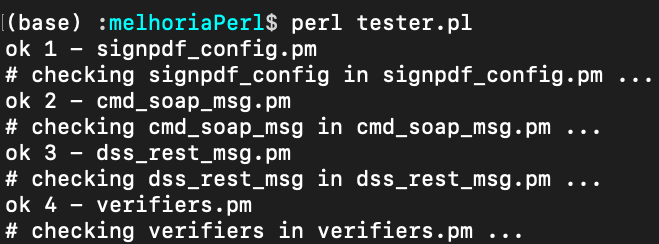
\includegraphics[scale = 0.25]{testvars.png}
  
  \caption {Verificação de variáveis não utilizadas nos ficheiros do programa}

\end{figure}
\par Como se pode verificar não existe a presença de variáveis por utilizar nos ficheiros do programa.


\subsubsection{SonarQube}
\hfill\newline

\par Após todo o trabalho levado a cabo para corrigir qualquer falha no código do programa, utilizei o SonarQube\cite{sonarQube} com uma extensão para Perl\cite{perlSonarQube} para confirmar mais uma vez que o código está de facto bem escrito e não possui duplicações ou outros problemas. O resultado de correr este programa de validação e deteção de Code Smells sobre o nosso programa pode ser visualiado na figura a baixo apresentada.

\begin{figure}[H]

  \centering
  \captionsetup{justification=centering}

  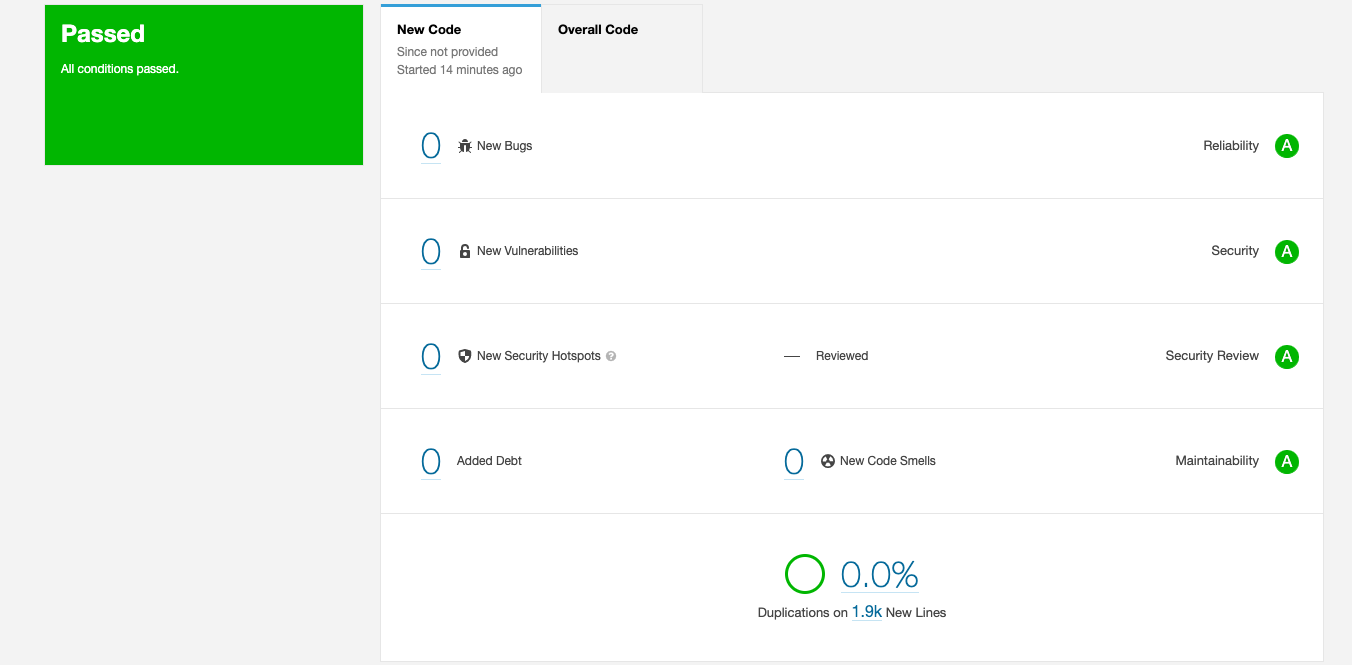
\includegraphics[scale = 0.25]{sonarQube.png}
  
  \caption {Relatório gerado pelo SonarQube sobre todos os ficheiros do programa}

\end{figure}

\par Claramente o programa não possui mais code Smells a serem retirados. Adicionalmente podemos verificar que, de facto, termos utilizado severidade de nivel 3 na análise recorrendo ao módulo \textit{Perl::Critic} foi a escolha certa uma vez que o addOn usado no SonarQube para verificar o código perl apresenta uma utilização refinada de vários módulos\cite{develCover,perlCritic} e regras de livros perl\cite{codeSmells2,livro1,livro2,livro3,bestpractices}. 

\subsection{Testes}

\par Para realizarmos testes sobre a aplicação, temos de verificar de que forma a podemos comprometer. A forma que temos de tentar realizar um ataque é através da inserção de inputs maliciosos, que podem ser introduzidos quando se passam argumentos no inicio programa ou no seu decorrer ou então quando o programa recebe uma resposta do servidor. Note-se que apesar de os inputs serem recebidos, todos sem exceção são enviados a alguma sub-rotina do módulo \textit{verifiers.pm} para verificação. Assim, para testar a robustez do programa basta tentar obter um resultado inesperado nos testes do módulo \textit{verifiers.pm} quando este deveria alertar para um erro de input, para este fim realizamos um fuzzing com recurso ao módulo \textit{Test::LectroTest}\cite{testelectro}. Este módulo permite definir propriedades que definem o tipo de inputs a passar ás funções a testar e o tipo de resposta esperado para esses inputs, adicionalmente, podemos criar uma mensagem informativa sobre a propriedade que está a ser testada.
\par Cada um dos inputs das propriedades supramencionadas pode ser definido como um tipo de variável, sendo que o módulo gerará esse input automaticamente ou alternativamente é possível criar um gerador para o input declarado, isto dá jeito quando, por exemplo, ao invés de uma string aleatória queremos uma string que contenha apenas letras minúsculas.
\par Foi por isso criada uma propriedade para cada verificação individual realizada no módulo \textit{verifiers.pm} que é testada sobre os inputs fornecidos e para cada input foi criado um gerador que permite testar um parte da sub-rotina de verificação. Tomemos por exemplo os geradores, a propriedade definida e e validação dos outputs da sub-rotina \textit{valid\_response()}. O primeiro passo para conseguirmos definir uma propriedade sobre esta é entender o seu funcionamento.
\begin{figure}[H]

  \centering
  \captionsetup{justification=centering}

  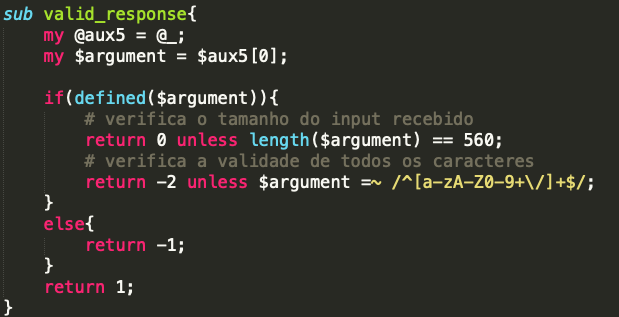
\includegraphics[scale = 0.25]{validateResponse.png}
  
  \caption {Sub-rotina valid\_response()}

\end{figure}
\par Esta começa por verificar se o valor recebido está definido, caso não esteja devolve -1, o que permitirá ao corpo principal do programa escrever a mensagem informativa: \textit{"Response not defined!"} antes de terminar. Caso a variável esteja definida temos 3 opções, a primeira é a variável não ter o comprimento certo, isto pode ser resultado de uma interseção da mensagem por parte de terceiros e consequente alteração do tamanho da mesma quer por truncação quer por adição, a sub-rotina prontamente devolve o código de erro 0 que permite mostrar ao utilizador a mensagem \textit{"Illegal length found on Response!!"} . A segunda hipótese prende-se com a alteração dos valores da mensagem de forma a inserir código com fins nefastos, assim é realizada uma verificação que garante que os caracters da mensagem são todos de base 64, caso não sejam esta sub-rotina devolve o valor de erro -2 que permite mostrar a seguinte mensagem de erro ao utilizador: \textit{"Wrong charaters on Response!!"}. Por fim temos a terçeira opção que assume que ao passar pelas várias validações o input é o original e está correto e portanto devolve o código 1 que permite que o programa avance. Assim, o nosso objetivo é fornecer um input que supostamente deva falhar uma verificação ou passar todas e cujo código devolvido não seja o esperado. O código desenvolvido com este intuito apresenta~se em seguida.


\begin{figure}[H]

  \centering
  \captionsetup{justification=centering}

  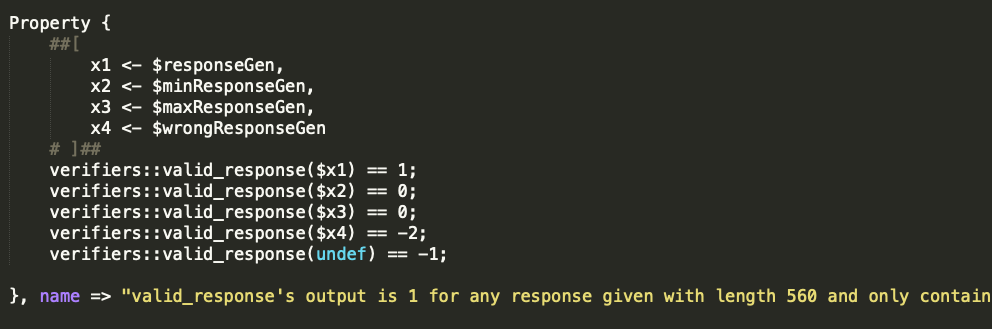
\includegraphics[scale = 0.3]{validateResponseTester.png}
  
  \caption {Propriedade que testa outputs da sub-rotina valid\_response()}

\end{figure}

Com se pode ver na imagem acima temos dentro da propriedade 4 inputs declarados com a sintax do módulo \textit{Test::LectroTest} e para cada input temos uma chamada á sub-rotina a testar. Os geradores destes inputs são apresentados em seguida bem como qual a propriedade que o input gerado pretende testar.
\begin{enumerate}
	\item String( charset=>"A-Za-z0-9+/", length=>[560])
	\par Este gerador gera uma mensage em base 64 que deve passar todos os testes de validação de input. A validação deve retornar sempre 1.\newline
	\item String( charset=>"A-Za-z0-9+/", length=>[561,])
	\par Este gerador gera mensagens cujos caracters são válidos em base 64 mas cujo tamanho é superior ao esperado. A validação deve retornar sempre 0.\newline
	\item String( charset=>"A-Za-z0-9+/", length=>[1,559])
	\par Este gerador gera mensagens cujos caracters são válidos em base 64 mas cujo tamanho é inferior ao esperado. A validação deve retornar sempre 0.\newline
	\item String( charset=>"[\&\%\$\#@"!?',;.:-\_ªº\textasciitilde\^{}\textbackslash\textbar]", length=>[560])
	\par Este gerador gera mensagens cujos caracters são inválidos em base 64 mas cujo tamanho é o esperado. A validação deve retornar sempre -2.
\end{enumerate}

Adicionalmente testaram-se também as respostas da validação a um input indefinido que, como previsto, retornou -1.

\par O mesmo tipo de raciocinio foi aplicada a cada sub-rotina do módulo \textit{verifiers.pm} e, no fim, as propriedades desenvolvidas foram aplicadas 10000 vezes, ou seja um número de vezes significativo para minimizar as hipóteses de terem sido gerados apenas inputs que favoreçam o intuito de cada propriedade e as avaliem como corretas. O resultado apresenta-se em baixo.


\begin{figure}[H]

  \centering
  \captionsetup{justification=centering}

  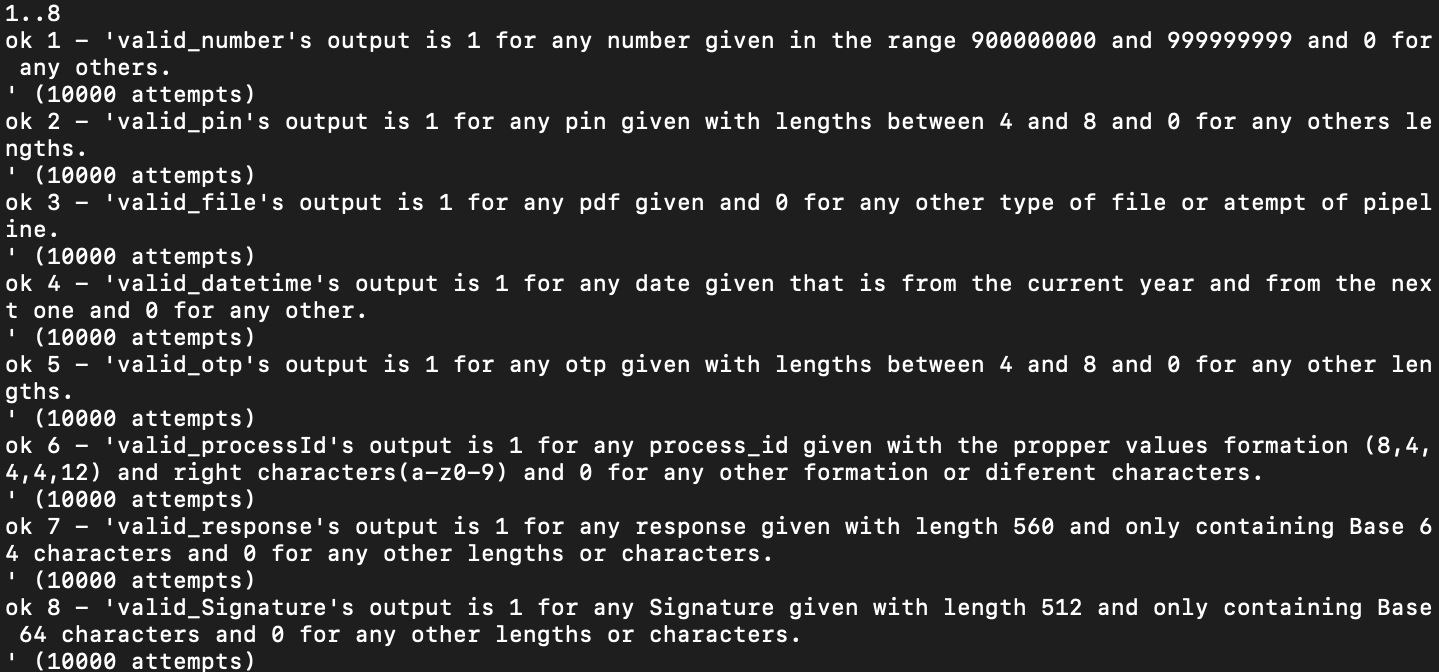
\includegraphics[scale = 0.25]{validations.png}
  
  \caption {Resultado das 10000 verificações utilizando cada uma das propriedades definidas}

\end{figure}




\newpage
\section{Como correr o programa}

\subsection{Módulos}
\par Antes de podermos correr o programa precisamos de ter os módulos requiridos pelo mesmo instalados. Para instalar os módulos necessários pode-se utilizar uma ferramenta chamada \textit{cpanm}\cite{cpanm}. Pode-se descarregar esta ferramenta para linux com o comando de terminal \textit{sudo apt install cpanminus}.\newline
Após instalar a ferramenta deve-se garantir que se têm os seguintes módulos instalados\footnote{Nota: Para descarregar os módulos use no terminal o comando cpanm install 'nome do módulo'}:

\begin{enumerate}
	\item Crypt::OpenSSL::X509
	\item DateTime
	\item Digest::SHA
	\item MIME::Base64
	\item Getopt::Long
	\item POSIX
	\item List::MoreUtils
	\item Carp
	\item FindBin
	\item IO::Prompt
	\item REST::Client
	\item XML::Compile::WSDL11
	\item XML::Compile::SOAP11
	\item XML::Compile::Transport::SOAPHTTP
	\item Encode
	\item Bit::Vector
	\item HTTP::Request
	\item HTTP::Parser
	\item Log::Log4perl
	\item LWP::ConsoleLogger
	\item strict
\end{enumerate}

Agora que temos os módulos necessários instalados podemos correr o programa e para  o fazer temos várias opções. Para saber qual a sintaxe pela qual o programa se rege deve-se chamar o programa seguido do argumento -h:
\begin{itemize}
	\item perl signpdf\_cli.pl -h
\end{itemize} 
\hfill\newline
O programa requer sempre 3 inputs obrigatórios:
\begin{itemize}
	\item Número de telemóvel do utilizador
	\item Pin da chave móvel digital
	\item Nome do pdf a assinar
\end{itemize}
\hfill\newline
Adicionalmente o programa permite ao utilizador fornecer 2 inputs extra \textit{Output file} e \textit{Datetime} que são respetivamente o nome a ser atribuido ao pdf assinado e a data a usar para assinar o mesmo, podendo o utilizador escolher fornecer apenas o primeiro, apenas o segundo ou ambos.\newline
Assim, apresentam-se em seguida as várias combinações disponíveis para a utilização da app:
\begin{enumerate}
	\item perl signpdf\_cli.pl -u '+351 XXXXXXXXX' -p XXXX -infile 'nome do ficheiro'.pdf
	\item perl signpdf\_cli.pl -u '+351 XXXXXXXXX' -p XXXX -infile 'nome do ficheiro'.pdf - outputfile 'nome do ficheiro'.pdf
	\item perl signpdf\_cli.pl -u '+351 XXXXXXXXX' -p XXXX -infile 'nome do ficheiro'.pdf -datetime YYYY-MM-DDTHH:MM:SS.SSSSSS
	\item perl signpdf\_cli.pl -u '+351 XXXXXXXXX' -p XXXX -infile 'nome do ficheiro'.pdf - outputfile 'nome do ficheiro'.pdf -datetime YYYY-MM-DDTHH:MM:SS.SSSSSS
\end{enumerate}


Caso corra a aplicação como um utilizador regular (sem debug) o resultado esperado é o seguinte:
\begin{figure}[H]

  \centering
  \captionsetup{justification=centering}

  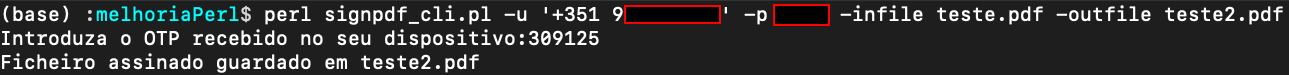
\includegraphics[scale = 0.25]{resultado1.png}
  
  \caption {Resultado de correr o programa sem o modo debug}

\end{figure}


 Caso corra a aplicação em modo debug poderá ver a forma dos envelopes enviados bem como a informação que circula nos seus headers e os seus conteúdos, o resultado esperado é o seguinte:

\begin{figure}[H]

  \centering
  \captionsetup{justification=centering}

  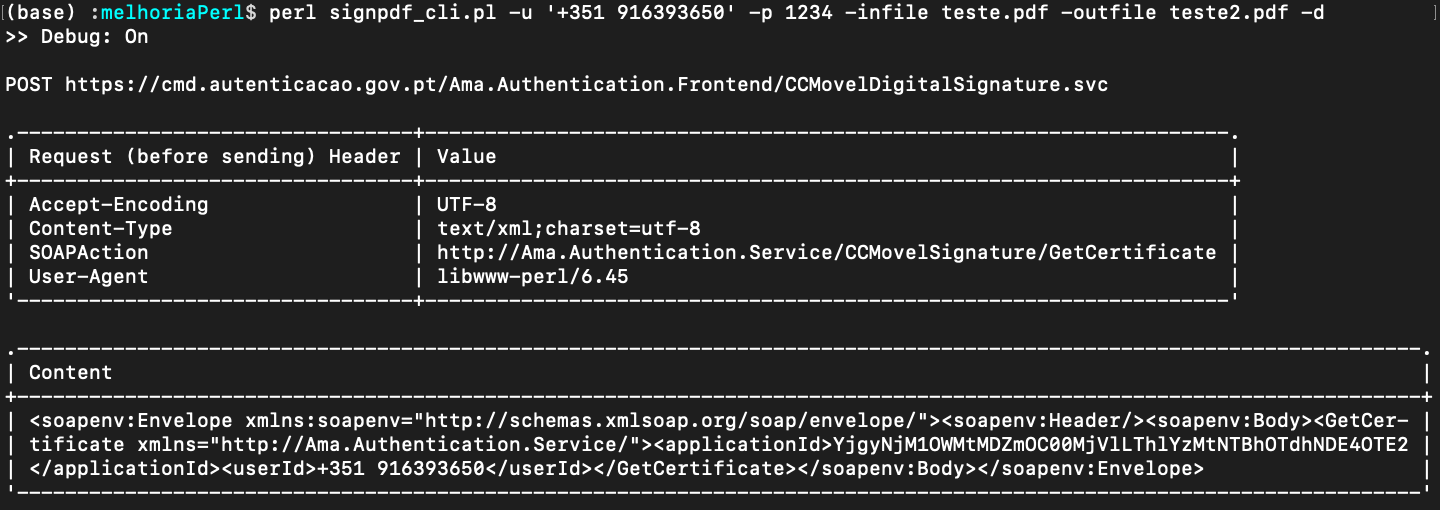
\includegraphics[scale = 0.25]{resultado2.png}
  
  \caption {Resultado de correr o programa com o modo debug}

\end{figure}
\newpage
\subsection{Replicação de testes}

Caso se pretendam replicar os testes realizados sobre a aplicação é necessário instalar alguns programas bem como alguns módulos do perl. Os módulos a instalar são os seguintes:

\begin{enumerate}
	\item Devel::Cover
	\item Perl::Critic
	\item Test::Vars
	\item Test::LectroTest
\end{enumerate}
Igualmente é necessário instalar os seguintes programas e bibliotecas (os links para obter os elementos listados também são fornecidos). Cada um dos elementos possui documentação para auxiliar a sua instalação e configuração:
\begin{enumerate}
	\item SonarQube (sonarqube.org)
	\item Biblioteca Perl para o SonarQube (https://github.com/sonar-perl/sonar-perl)
	\item Sonar-Scanner para o SonarQube (https://docs.sonarqube.org/latest/analysis/scan/sonarscanner/)
\end{enumerate}

Após a instalação dos recursos supramencionados basta analisar o programa criado com os mesmos, seguindo os passos referidos na \autoref{sec:Testes}.





\newpage

%
% ---- Bibliography ----
%
% BibTeX users should specify bibliography style 'splncs04'.
% References will then be sorted and formatted in the correct style.
%
% \bibliographystyle{splncs04}
% \bibliography{mybibliography}
%
\begin{thebibliography}{8}

%\bibitem{ref_intro1}
%https://www.itu.int/en/ITU-D/Statistics/Pages/stat/default.aspx
\bibitem{ref_intro1} http://perlcritic.com/critique/file
\bibitem{ref_intro2} https://github.com/Hack-with-Github/Awesome-Hacking
\bibitem{ref_intro3} https://metacpan.org/pod/Date::Manip::Range
\bibitem{sonarQube} https://docs.sonarqube.org/latest/analysis/overview/
\bibitem{perlSonarQube} https://github.com/sonar-perl/sonar-perl
\bibitem{lwpUserAgent} https://metacpan.org/pod/LWP::UserAgent
\bibitem{lwpConsoleLoger} https://metacpan.org/pod/LWP::ConsoleLogger
\bibitem{codeSmells1} https://blog.codinghorror.com/code-smells/
\bibitem{codeSmells2} Martin Fowler, Kent Beck. \textit{Refactoring - Improving the Design of Existing Code}. Addison-Wesley Professional; November 30, 2018.
\bibitem{develCover} https://metacpan.org/pod/Devel::Cover
\bibitem{perlCritic} https://metacpan.org/pod/Perl::Critic
\bibitem{perllist} https://metacpan.org/pod/List::MoreUtils
\bibitem{ioPrompt} https://metacpan.org/pod/IO::Prompt
\bibitem{testVars} https://metacpan.org/pod/Test::Vars
\bibitem{livro1} Peteris Krumin. \textit{Perl One-liners}. No Starch Press, Inc.
\bibitem{livro2} \textit{Perl - Notes for Professionals}.
\bibitem{livro3} Peter Wainwright, Aldo Calpini, Arthur Corliss Simon Cozens, Juan Julián Merelo, Guervós Chris Nandor, Aalhad Saraf. \textit{Professional Perl Programming}. Wrox Press Ltd.
\bibitem{livro4} Tom Christiansen, Nathan Torkington. \textit{Perl Cookbook}. O’Reilly Media, Inc.
\bibitem{bestpractices} Damian Conway. \textit{Perl Best Practices}. O'Reilly Media, Inc.
\bibitem{testelectro} https://metacpan.org/pod/Test::LectroTest
\bibitem{cpanm} https://metacpan.org/pod/App::cpanminus
\end{thebibliography}
%\input{anexo.tex}

\end{document}